% Chapter 1

\chapter{Introduction} % Main chapter title

\label{Chapter1} % For referencing the chapter elsewhere, use \ref{Chapter1} 

Memory corruption errors have been a big security problem for almost 40
years~\cite{szekeresSoKEternalWar2013,vanderveenMemoryErrorsPresent2012}. The
errors offtenly happen due to the use of unsafe languages, mainly C and C++ in
building applications. This safety issue becomes a significant attack surfaces
that affect the security of many critical applications. The adversaries can
hijack the program and taking the control to achieve their goals. Such attack
gives impact to wide range applicatinos from distributed systems running in the
cloud to IoT devices that are ubiquitous nowadays.

Since the identification these vulnerabilities, a continues arm races have been
ongoing between adversaries and defenders. As attackers find a vulnerability
then a different defense mechanisms is invented. After that, attackers and
researchers find another vulnerability that can circumvent or disable the
defense. Or sometime, the solutions are not just practical to be deployed.
Across the year we are having solution such as non-executable stack (NX) or Data
Execution Prevention (DEP)  \( W \bigoplus R
\)~\cite{vanderveenMemoryErrorsPresent2012} Control Flow Integrity
(CFG)~\cite{abadiControlFlowIntegrityPrinciples2005},
ASLR~\cite{kilAddressSpaceLayout2006}, Stack
Canaries~\cite{baratlooTransparentRunTimeDefense2000} and more. Unfortuantely
the war is not over.

In 2016, Abera et al published a solution called C-Flat for detecting a
control-flow attack in runtime~\cite{aberaCFLATControlFlowAttestation2016}. The
detection is performed by mechanism called remote
attestation~\cite{haldarSemanticRemoteAttestationA2004}. The research focused on
attesting runtime control-flow attack on IoT or other embedded devices. Since
then, many different runtime remote attestation schema are
introduced~\cite{dessoukyLOFATLowOverheadControl2017,
zeitouniATRIUMRuntimeAttestation2017, kohnhauserSCAPIScalableAttestation2017,
dessoukyLiteHAXLightweightHardwareassisted2018, aberaDIATDataIntegrity2019,
koutroumpouchosSecureEdgeComputing2019, sunOATAttestingOperation2020}. Like
C-Flat, most of those remote attestation scheme are targetting embedded systems.
One unique runtime remote attestation schema name ScaRR tries to cover remote
attestation beyond embedded application but also made it work for complex
system~\cite{toffaliniScaRRScalableRuntime2019}. 

This thesis study different model for runtime remote attestation. We zoom in the
ScaRR implementation due to the unique strength on making the attestation work
for complex system.

\section{Motivation}

In this thesis we want to answer these questions.
\begin{itemize}
    \item What are different remote attestation model that is available now and
    how do they differ?
    \item How to implement offline program analysis for the ScaRR novel model
    for remote attestation?
    \item How is the performance of the model?
\end{itemize}

\section{Related Works}

\ft{too many images, it is not a comics! -- remove the images}
In this section, we discuss on the different runtime remote attestation
model. Specifically we discuss how different attestation scheme encode the
offline program representations.

C-Flat~\cite{aberaCFLATControlFlowAttestation2016} is the first remote
attestation scheme to detect runtime control flow attack for embedded systems.
Figure~\ref{fig:c-flat} shows how C-Flat generates offline measurement by
traversing all possible path of program from start node to the termination node.
In each node, C-Flat hashes the node ID and the hash of previous node. In the
first node, since there is no previous hash, we pass 0. This creates hash chains
which is stored as offline measurement database.

\begin{figure}[htbp]
\centerline{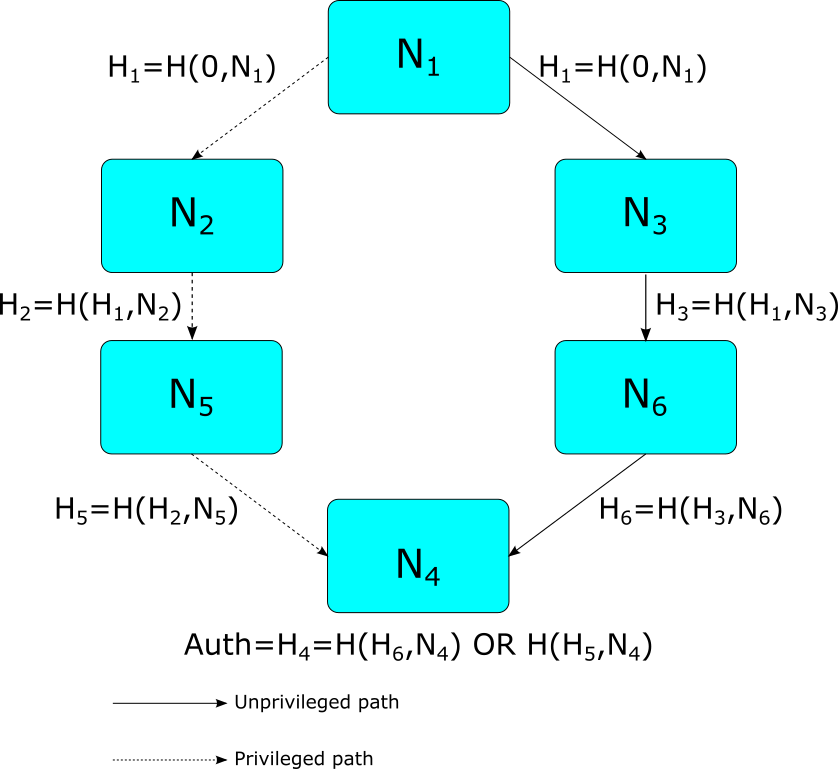
\includegraphics[scale=.5]{Figures/01/cflat-overview.png}}
\caption{C-Flat}
\label{fig:c-flat}
\end{figure}

With that control-flow model, C-Flat can attest the exact control-flow path of
the program. C-Flat also doesn't need source code because the offline
measurement can be run on the binary program. However, C-Flat has one limitation
---which is stated by the authors themselves--- on its inefficiencies for having
to explore all possible path from program control flow
graph~\cite{aberaCFLATControlFlowAttestation2016}.

\begin{figure}[htbp]
\centerline{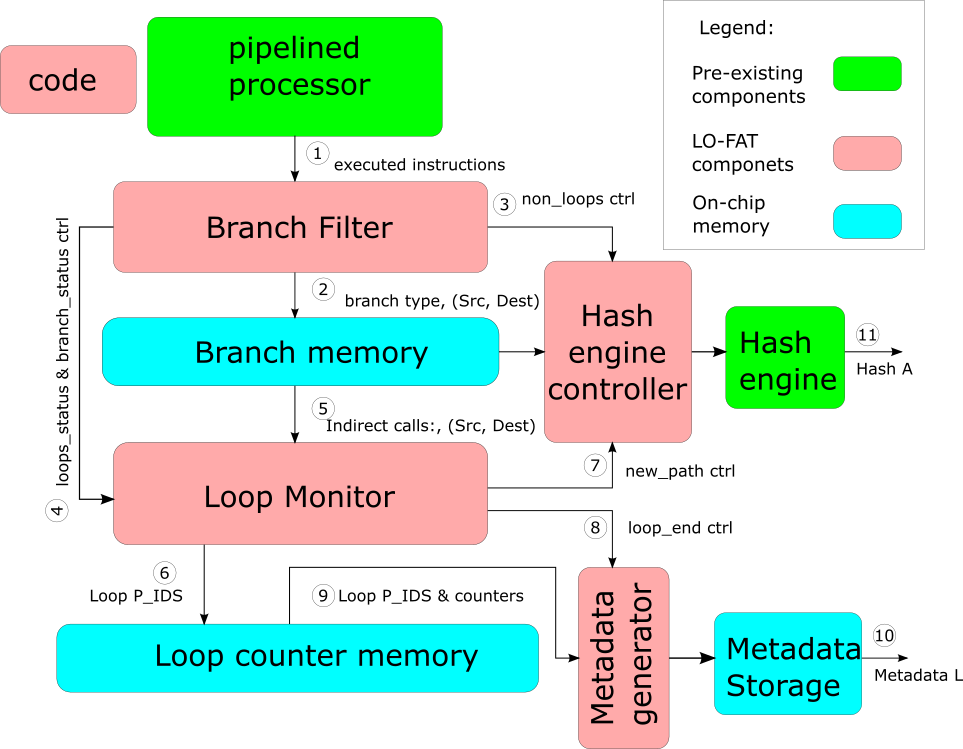
\includegraphics[scale=.5]{Figures/01/lofat-overview.png}}
\caption{Lo-Fat}
\label{fig:lo-fat}
\end{figure}

Lo-Fat~\cite{dessoukyLOFATLowOverheadControl2017} improves C-Flat by using
hardware support for control flow attestation. See Figure~\ref{fig:lo-fat} for
the Lo-Fat architecture. The hardware will intercept the instructions and
process it in the components called branch filter and loop monitor. With this
hardware support, Lo-Fat incurs no performance overhead. However, Lo-Fat
control-flow representation still inherits C-Flat approach, therefore it still
induce high verification cost.

Atrium~\cite{zeitouniATRIUMRuntimeAttestation2017} is remote attestation scheme
that can provide resiliency against physical memory attack where adversaries can
exploit the property of Time of Check Time of Use (TOCTOU) during attestation.
In this paper author are describing memory bank attack where adversary can
control instruction fetches to benign memory area when attestation is running
and direct the fetch to the malicious area otherwise.

\begin{figure}[htbp]
\centerline{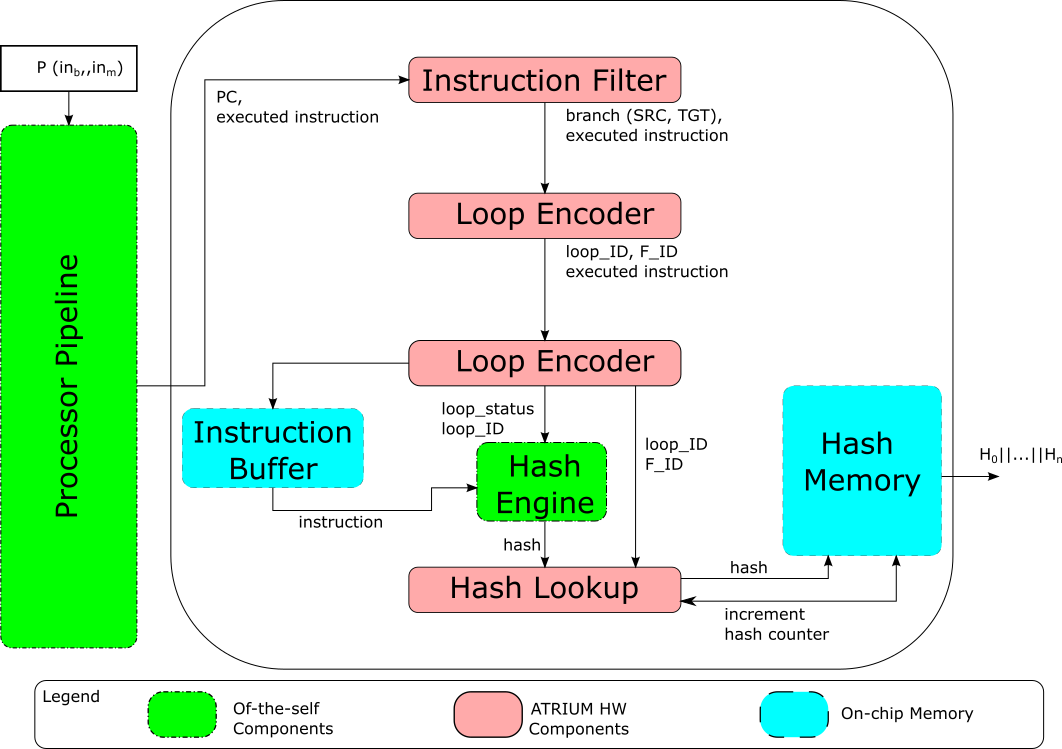
\includegraphics[scale=0.5]{Figures/01/atrium-overview.png}}
\caption{Atrium Architecture}
\label{fig:atrium}
\end{figure}

The offline measurement are calculated slightly different compared with C-Flat
and Lo-Fat. In Atrium, the verifier perform one-time pre-processing to generate
CFG of the program and computes cryptographic hash measurement over the
instructions and addresses of basic blocks. C-Flat are only hash the node ID.
While this approach can mitigate the TOCTOU attack, the offline measurement
generation still grow exponentially as the complexity of the program grow. 

LiteHax~\cite{dessoukyLiteHAXLightweightHardwareassisted2018} is hardware
assisted remote attestation scheme that allow verifier to detect these different
attacks:

\begin{itemize}
    \item control-data attack such as code injection or code reuse attack like ROP
    \item non-control-data attack
    \item data-only attack such us DOP which do not affect control flow
\end{itemize}

Different with the previous remote attestation scheme, the offline measurement
phase of LiteHax are only generates program CFG without calculating any hash
over all control flow and data flow events. However, in the online prover-side
verification time, prover are still computing hash and sending it as report to
the verifier. Verifier runs symbolic execution and incremental forward data-flow
analysis without doing any lookup to offline measurement database. LiteHAX
architecture can be seen in figure~\ref{fig:litehax}.

\begin{figure}[htbp]
\centerline{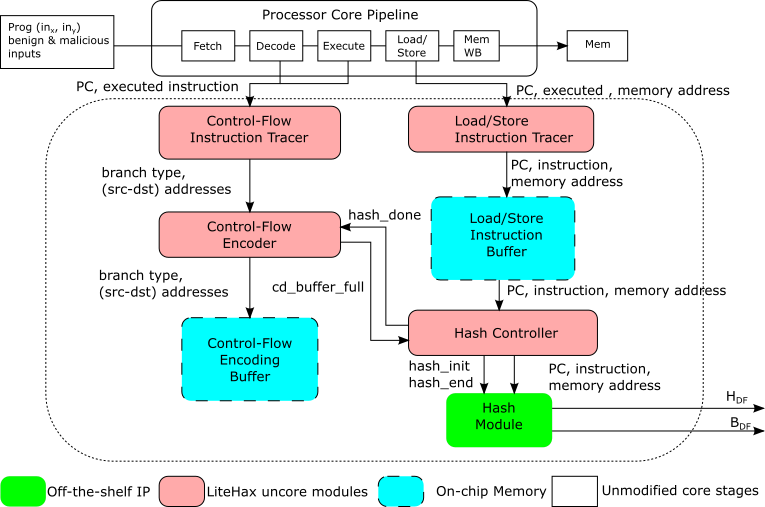
\includegraphics[scale=0.75]{Figures/01/litehax-overview.png}}
\caption{LiteHAX Architecture}
\label{fig:litehax}
\end{figure}

Diat~\cite{aberaDIATDataIntegrity2019} is remote attestation scheme that can
attest data integrity and control-flow of autonomous collaborative network
systems. To improve efficiency of attestation, the program attested must be
decomposed into small interacting modules. Data-flow monitoring is to be setup
between critical modules. Control path attestation is being done against novel
execution path representation using multiset has (MSH)
function~\cite{clarkeIncrementalMultisetHash2003}. See the control flow monitor
logic in figure~\ref{fig:diat}. The use of MSH makes some execution order of the
program cannot be reconstucted.

\begin{figure}[htbp]
\centerline{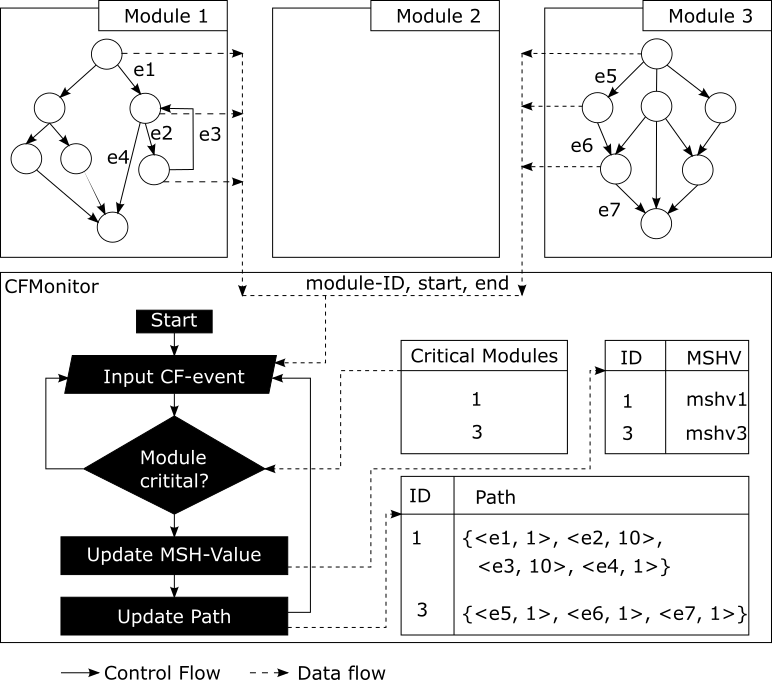
\includegraphics[scale=.5]{Figures/01/diat-cfmonitort.png}}
\caption{Diat CFMonitor Logic}
\label{fig:diat}
\end{figure}

\begin{figure}[htbp]
\centerline{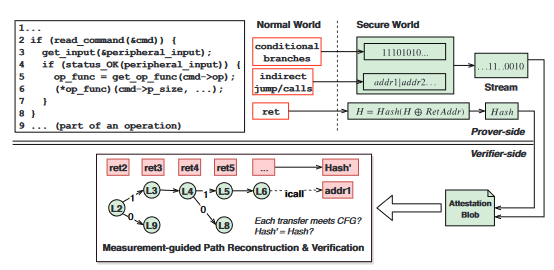
\includegraphics[scale=.85]{Figures/01/oat.png}}
\caption{OAT Control-Flow Attestation}
\label{fig:oat}
\end{figure}

OAT~\cite{sunOATAttestingOperation2020} is remote attestation scheme to attest
operation integrity of embedded device. OAT defines two type of measurements for
control flow attestation: a trace (for recording branches and jumps) and a hash
(for encoding returns). These two measurements are encoded as $H = Hash(H
\bigoplus RetAddr)$ which called as attestation blob. Figure~\ref{fig:oat} shows
the OAT control-flow attestation.

During verification, verifier reconstruct paths from the attestation blob. The
control flow violation is identified when CFI check against an address is failed
or mismatched between hash and trace.

Although OAT does not encounter the combinatorial hash explosion in C-Flat,
there is a verification overhead since verifier needs to reconstruct the
attestation blob. 
